\documentclass{acm_proc_article-sp}

\usepackage{graphicx}
\usepackage{listings}
\usepackage{epsfig}
\usepackage[all]{xy}

\begin{document}
\lstset{language=Haskell, numbers=left,
numberstyle=\tiny,numbersep=5pt,basicstyle=\scriptsize,aboveskip=20pt}

\title{Scenario Variability as Crosscutting}


\numberofauthors{2}

\author{
\alignauthor
Rodrigo Bonif\'{a}cio\\
       \affaddr{Informatics Center}\\
       \affaddr{Federal University of Pernambuco}\\
       \affaddr{Recife, Brazil}\\
       \email{rba2@cin.ufpe.br}
\alignauthor
Paulo Borba\\
       \affaddr{Informatics Center}\\
       \affaddr{Federal University of Pernambuco}\\
       \affaddr{Recife, Brazil}\\
       \email{phmb@cin.ufpe.br}
}

\maketitle              

\begin{abstract}
Variability management is a common challenge for Software Product
Line (SPL) adoption, since developers need suitable
mechanisms for describing or implementing different kinds of variability
that might occurs at different SPL views (requirements, design,
implementation, and test). In this paper, we present a framework for
modeling use case scenario variability mechanisms, enabling a better
separation of concerns between languages used to manage
variabilities and languages used to specify use case scenarios. The
result is that both representations can be understood and evolved in
a separated way. We achieve such goal by modeling variability management
as a crosscutting phenomenon, for the reason that features often affect
different points of each SPL view. Additionally, we believe that our proposed framework might be customized to 
describe variability mechanisms in other SPL artifacts, being a contribution for automatic product generation and traceability.
\end{abstract}

\category{D.2.1}{Software Engineering}{Requirements}[Languages,
Methodologies]\
\category{D.2.13}{Software Engineering}{Reusable
Software}

\terms{Design, Documentation}

\keywords{Software product line, variability management, requirement models}

%
\section{Introduction}
%
The support for variation points enables product
customization from a set of reusable
assets~\cite{phol-spl-book}. However, variability management, due to
its inherent crosscutting nature, is a common challenge in software
product line (SPL) adoption~\cite{northrop-spl-book,phol-spl-book}.
Such crosscutting characteristic is materialized whenever a feature
requires variation points to be spread in different SPL artifacts. Actually, 
the representation of a variant feature is often spread not only 
in several artifacts, but also at the different product line views (requirements, 
design, implementation, and test). In this case, variability management, in 
the same way as the feature model and the architecture, represents a central concern in the SPL 
development and should not be tangled with existing artifacts~\cite{phol-spl-book}.   
 
Several authors have proposed the use of \emph{aspect-oriented} mechanisms in order to better modularize variability management at source code~\cite{alves-gpce-06,mmedeiros-lawasp-2007}. However, to our knowledge, no attempt has been done to verify which are the crosscutting mechanisms that could be applied for managing variabilities at requirements, design, and test artifacts. Actually, current techniques for scenario variability management~\cite{favaro-icsr-98,bertolino-esec-2003,eriksson-splc-2005} do 
not present a clear separation between variability management and scenario specification. For instance, supposing that  product variants are tangled with  use case scenarios, if one variant is removed from the product line, it would be necessary to change all related scenarios. In summary, it is difficult to evolve both representations. 

Another problem is the lack of a formal representation for the weaving processes used 
to derive product specific scenarios. This is not suitable for current SPL generative 
practices~\cite{krueger-cacm-200712}; following the aforementioned works, it is difficult to automatically derive 
the requirements of a specific SPL member and to check if the specified compositions 
between basic and variant flows are correct.  Although  the semantic composition of PLUC (Product 
Line Use Case)~\cite{bertolino-esec-2003} is defined in~\cite{fantechi-splc-2004}, such approach 
does not separate scenario specification from variability management. In order to explain in more details 
the problems addressed by this work, a motivating example is presented  in Section~\ref{sec:example}.  

In this paper, we describe a framework for modeling the composition 
process of scenario variabilities (Section~\ref{sec:models}). 
Such framework aims to: (1) represent a clear separation between variability management 
and scenario specification; and (2) specify how to weave these representations in order to generate
specific scenarios for a SPL member. Therefore, the main contributions of this work are

\begin{itemize}

\item A formal characterization of variability management as a crosscutting concern and, in this way, enforce that it  
must be represented as an independent view of the SPL. Although this work focus on requirement artifacts, 
more specifically use case scenarios, we argue that such separation is also valid for other SPL views. Actually,
it has already been claimed for source code~\cite{alves-gpce-06,mmedeiros-lawasp-2007}.
  
\item A framework for modeling the composition process of scenario variability mechanisms. 
This framework gives a basis for describing variability mechanisms, 
allowing a better understanding of each mechanism. In this work, such framework is used for modeling 
the semantics of scenario variation mechanisms, but it might be customized for other SPL views.

\item Describe three scenario variation mechanisms using the
modeling framework. Such descriptions present
a more formal representation when compared to existing works; this is an
important property for supporting the automatic derivation of product
specific artifacts.

\end{itemize}

Since our modeling framework is based on Masuhara and Kiczales work~\cite{kiczales-ecoop-2003}, another 
contribution of this paper is that we have applied their definition about \emph{what} characterize a mechanism as crosscutting in the domain of variability management. Based on their view of crosscutting, we can reason about variability management as a crosscutting concern that weaves different input specifications in order to derive a product specific member. 

Finally, we evaluate our approach (Section~\ref{sec:evaluation}) by comparing it 
to existing works and observing a set of three criteria: support for the 
different kinds of variability, separation of concerns, and design expressiveness.  We 
also relate our work with other research topics (Section~\ref{sec:related}) and present our concluding 
remarks in Section~\ref{sec:conclusions}.

%-----------------------------------------------------------------------
% Subsection: Motivating example
%-----------------------------------------------------------------------
\section{Motivating Example}
\label{sec:example}

In order to customize specific products, by selecting a valid feature configuration, variant points must be represented in the 
product line artifacts. Several variant notations have been proposed for use case scenarios, like  Product Line Use Cases (PLUC)~\cite{bertolino-esec-2003} and Product Line Use Case Modeling for Systems and
Software Engineering (PLUSS)~\cite{eriksson-splc-2005}. However, besides
the benefits of variability support, existing works do not present a clear separation between variability 
management and scenario specifications. In this section we illustrate the resulting problems 
using the \emph{eShop Product Line}~\cite{eshop-url} as a motivating example. 

The main use cases of the \emph{eShop Product Line} (EPL) 
allow the user to \emph{Register as a Customer}, \emph{Search for Products}, 
and \emph{Buy Products}.  Five variant features are described in the original specification,
allowing a total  of 72 applications to be derived from the product line~\cite{eshop-url}. Here, 
we consider extra features, such as \emph{Update User Preferences} that, based on the user historical data of searches 
and purchases, updates user preferences. Figure~\ref{fig:eshop-fm} presents part of the \emph{eShop} feature model~\cite{gheyi-alloy-06,czarnecki-book,kang-foda-report}. 
As a brief introduction about the feature model notation, the relationships between a parent and its child are 
categorized as: \emph{Optional} (features that might not be selected in a specific product), \emph{Mandatory} (feature that must be selected, if the parent is also 
selected), \emph{Or} (one or more subfeatures might be selected), and \emph{Alternative} (exactly one subfeature must be selected).     

 \begin{figure}[h]
 \begin{center}
  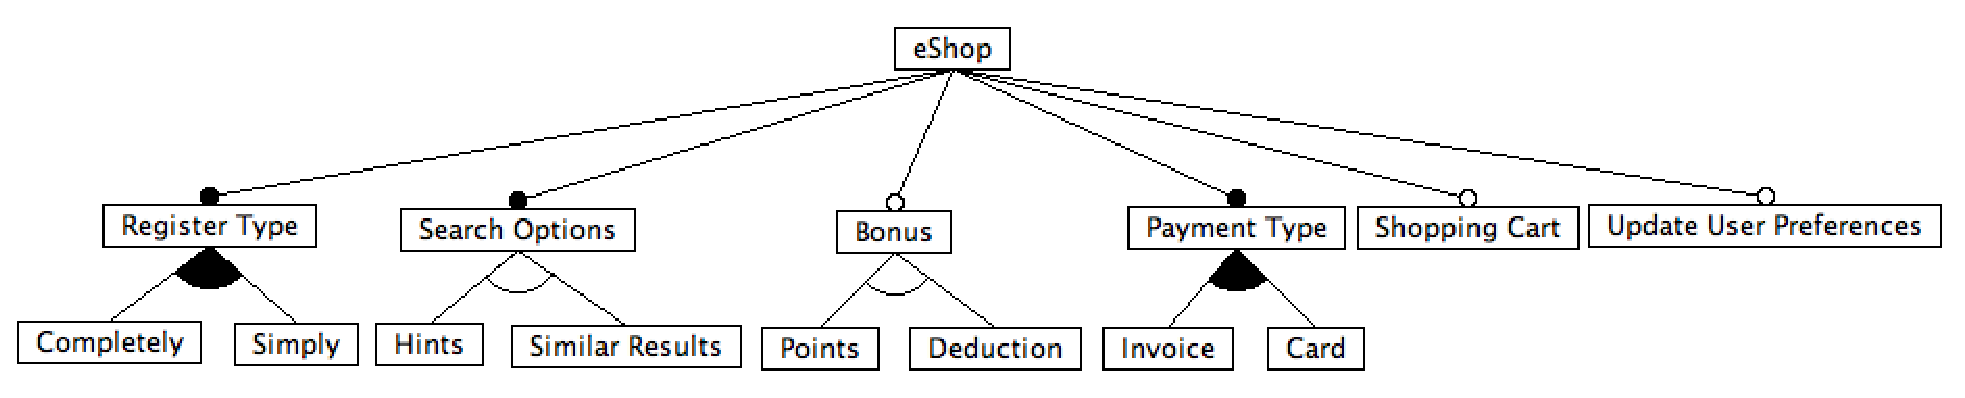
\includegraphics[scale=0.25]{img/eShop-fm3.eps}
   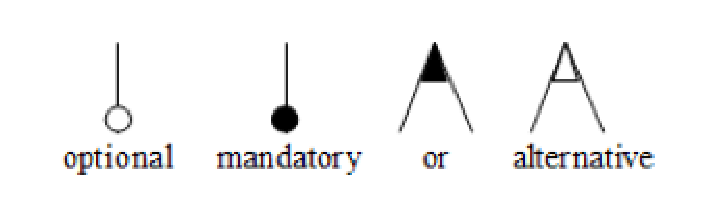
\includegraphics[scale=0.30]{img/fm-notation.eps}
  \caption{eShop feature model.}
  \label{fig:eshop-fm}
  \end{center}
\end{figure}


%Other approaches are based on use case extensions~\cite{jacobson-reuse-book}, not explored here since they 
%require that one use case extension must be defined for each variant. This can result in a huge
%number of use cases that is not suitable for managing activities.

In the PLUSS approach, all variant steps of a scenario specification are defined in the same artifact. For example, steps 1(a) and 1(b) in Figure ~\ref{fig:pluss-01} are 
never performed together. They are alternative steps: Step 1(a) will be present only if the \emph{Shopping Cart} feature is selected (otherwise Step 1(b) will be present). In a similar way, we have to choose between options (a) and (b) for Step 2 (depending on the \emph{Bonus Feature} has been selected or not). Finally, Step 6 is optional and will be present only if the feature \emph{Update User Preference} is selected. 


\begin{figure}[h]
\begin{center}
\begin{scriptsize}
  \texttt{
  \begin{tabular}{|p{0.2in}|p{1.3in}|p{1.3in}|}
   \hline
	Id    & User Action & System Response \\ \hline \hline    
       1(a) &Select the checkout option. & Present the items in the shopping cart and the amount to be paid. The user can remove items from shopping cart. \\  \hline
       1(b) & Select the buy product option. & Present the selected product. The user can change the quantity of item that he wants to buy. Calculate and show the amount to be paid. \\  \hline
       2(a) & Select the confirm option. & Request bonus and payment information. \\  \hline
       2(b) & Select the confirm option. & Request payment information. \\  \hline
       3     & Fill in the requested information and select the proceed option. & Request the shipping method and address.\\  \hline
       4     & Select the \$ShipMethod\$, fill in the destination address and select the proceed option. & Calculate the shipping costs. \\  \hline
       5     & Confirm the purchase. & Execute the order and send a request to the Delivery System in order to dispatch the products. \\  \hline
       6     & Select the close section option. & Register the user preferences.\\  \hline
  \end{tabular}
  } 
\end{scriptsize}
\caption{Buy Products scenarios using the PLUSS notation.}
\label{fig:pluss-01}
\end{center}
\end{figure}

Following this approach, it is hard to understand a specific configuration because all possible variants are described in the same artifact. Also, such tangling between variant representation and scenario specification results in maintainability issues: introducing a new product variant might require changes in several points of existing artifacts.  For example, including a \emph{B2B Integration} feature, which allows the integration between partners in order to share their warehouses, might change the specification of \emph{Buy Product} scenario, enabling the search for product availability in remote warehouses (a new variant for Step 1) and updating a remote warehouse when the user confirms the purchase (a new variant for step 5). Moreover, the inclusion of this new optional feature also changes the specification of \emph{Search for Products} scenario (the search might also be remote). In summary, since the behavior of certain features can be spread among several specifications and each specification might describe several variants, the efforts needed to understand and evolve the product line might increase.    

Instead of relating each variant step to a feature, PLUC introduces special tags for representing 
variabilities in use case scenarios. For example, the VP1 tag in Figure~\ref{fig:pluc-01}, which also 
describes the \emph{Buy Products} scenario, denotes a variation point that might assumes the 
values ``\emph{checkout}'' or ``\emph{buy item}'', depending on which product was configured. For 
each \emph{alternative} or \emph{optional} step, one tag must be defined. The actual value
of each tag is specified in the \emph{Variation Points} section of the scenario specification. 

\begin{figure}[h]
\begin{center}
\begin{scriptsize}
  \texttt{
  \begin{tabular}{{|p{0.05in}p{3in}|}}
  \hline
  & {\bf Buy Products Scenario} \\
  & {\bf Main Flow} \\
  01 & Select [VP1] option \\
  02 & [VP2] \\
  03 & Select the confirm option \\
  04 & [VP3] \\
  05 & Fill in the requested information and select the proceed option \\
  06 & Request the shipping method and address \\
  07 & Select the [VP4] shipping method, fill in the destination address and select the proceed option \\
  08 & Calculate the shipping costs. \\ 
  09 & Confirm the purchase. \\
  10 & Execute the order and sends a request to the Delivery System in order to dispatch the products \\  
  11 & Select the close section option. \\ 
  12 & \{[VP5] Register the user preferences.\} \\  & \\
  & {\bf Products definition: } \\ & VP0 = (P1, P2) \\ & \\
  & {\bf Variation points: } \\ 
  &  VP1 =  if (VP0 == P1) then (checkout) \\ & \hspace{0.25in} else (buy product) \\
  & VP2 =  if (VP0 == P1) \\ & \hspace{0.25in}  then (Presents the items in the shopping cart...) \\ & \hspace{0.25in} else (Present the selected product. The user...) \\
  & VP3 =  if (VP0 == P1) \\ & \hspace{0.25in} then ( Requests bonus and payment information.) \\ & \hspace{0.25in} else (Requests payment information.) \\
  & VP4 =  (Economic, Fast) \\
  & VP5 requires (VP0 == P1) \\ \hline
   \end{tabular}
  } 
\end{scriptsize}
\end{center}
\caption{Buy Products scenarios using the PLUC notation.}
\label{fig:pluc-01}

\end{figure}

A different kind of tangling occurs in this case, since segments of the specification are tangled with the variation 
points. Additionally, SPL members are also described using the same tag notation (see the \emph{Product Definition} section 
in Figure~\ref{fig:pluc-01}). There is no explicit relationship between product configurations and feature models. In the example, 
two products (P1 and P2) are defined. The first product is implicitly configured by selecting the \emph{Shopping Cart}, 
\emph{Bonus}, and \emph{Update User Preferences} features. The second model, instead, is not configured 
with such features. 

Since the values of alternative and optional variation points are computed based on the defined products, instead 
of specific feature, the inclusion of a new member in the product line might require a deeply review of 
variation points. Moreover, since the variation points and the product definitions are spread among several scenario specifications, it is hard and time consuming to keep the SPL consistent. Finally, the same definitions (product configuration and variation points) often are useful to manage variabilities in other artifacts, such as design and source code. As a consequence, this approach requires the replication of such definitions in different SPL views - if the SPL evolved, changes would be propagated throughout many artifacts.

In summary, both techniques rely on simple composition techniques: filtering variant steps in scenarios or syntactic changes of tag values based on product definition. In this sense, they are similar to conditional compilation techniques, which have been applied to implement variability at source code. Such techniques are not suitable for modularizing the crosscutting nature of certain features, has poor legibility, and leads to lower maintainability~\cite{alves-gpce-06}. 
Consequently, we argue that the variability management concern should be separated from the other artifacts and used as a language for generating specific products. The automatic generation of specific product artifacts has being recommended by the SPL community~\cite{krueger-cacm-200712,greenfield-softwarefactories,czarnecki-book}, in such way that the combination of generative techniques, aspect oriented programming, and software product line should be further investigated. In this case, in order to support the automatically derivation of product specific artifacts, it is necessary not only a more precise definition of each language used to describe product line artifacts and the variability management concern, but also the weave processes used to combine them. PLUSS and PLUC approaches fail in this direction, since Eriksson et al., although present the metamodel of PLUSS notation~\cite{eriksson-splc-2005}, do not describe which languages and processes are used for relating use case scenarios to feature models. Likewise, besides Fantechi et al. describe the formal semantics of PLUC~\cite{fantechi-splc-2004}, this approach does not separate variability management from use case scenarios.

The next section describes our approach that considers scenario variability as a composition of different artifacts. Although in this paper we are focus on use case scenarios, the idea of separating product line artifacts from variability management is also applied to other SPL views. Moreover, we believe that our modeling framework, which describes the weaving processes for handle variability management, might be customized for design, implementation, and test artifacts. 




%-------------------------------------------------------------------------
% Section: Scenario Variabilities
%------------------------------------------------------------------------
%\section{Scenario variabilities}
%\label{sec:req-var}

%Eriksson et al.~\cite{eriksson-splc-2005} presented
%four kinds of variabilities in use case models for product
%families: (i) use cases might be included
%in a given product ({\bf optional use cases}), (ii) certain
%scenarios of an included use case might be excluded from a
%particular product ({\bf optional scenarios}), (iii) the flow of
%events within an included scenario might vary ({\bf changing
%scenarios}), and (iv) crosscutting requirements might affect several
%use cases on several levels ({\bf crosscutting variability}).

%In order to illustrate examples of such variabilities, consider a Message Application Product Line (MAPL) used to create, receive, and 
%manage different kinds of message (such as e-mail, short messages, and multimedia messages) for mobile 
%devices. Depending on the target device, a specific member of the product line is composed by specific use case/scenario 
%configurations. Figure~\ref{fig:fm-01} depicts part of the Message Application feature model~\cite{czarnecki-book, czarnecki-
%wsfactory-2005, 
%kang-foda-report}, used for representing possible configurations 
%of the product line. For a better understanding of the example, we briefly introduce some features of the MAPL. 

%\begin{description}
%\item[Message Application (FEA01):] The MAPL root feature. This feature requires that some use cases must be present in all 
%members of the product line, such as \emph{Create and Send a Message} and \emph{Receive and Save a new Message} use cases.

%\item[Message Type (FEA02):] Feature used to represent the different kinds of messages (\emph{email}, \emph{sms}, \emph{mms}) 
%that might be supported by a product line member. At least one kind of message must be selected. 

%\item[Folder Management (FEA03):] Feature used to configure the folder management capabilities. Two kinds of folder management 
%are supported: single and multiple folders. If a product is configured with multiple folder support, the subscriber will be able to select 
%the place
%where a received message should be saved. Otherwise, the message must be saved on a specific folder (\emph{inbox folder}). 
%Multiple folder management also requires a specific use case (\emph{Manage Multiple Folders} use case) to \emph{create}, \emph
%{rename} and \emph{remove} folders and \emph{move messages} between folders. Additionally, Folder Management feature can be 
%configured as \emph{basic} or \emph{extended} size  (support for storing 1000 or 1500 messages).

%\end{description}
%  
%Suppose that if the feature \emph{Multiple Folders} is selected, 
%an extended version of \emph{Receive and Save a new Message} scenario
%and the \emph{Manage Multiple Folders} use case will be present in
%the target product (the basic version of \emph{Save a Message}
%scenario will not be present). In the SPL terminology, a
%\emph{configuration knowledge} should be used for describing 
%relationships between features and software artifacts
%(Table~\ref{tab:ck-01} is a simplified representation of a
%configuration knowledge). The variability related to the
%\emph{Manage Multiple Folders} use case is an example of optional
%use case variability. On the other hand, the \emph{basic} and
%\emph{extended} versions of \emph{Receive and Save a new Message} scenario compose an example of changing scenario 
%variability.

%\begin{figure}[h]
% 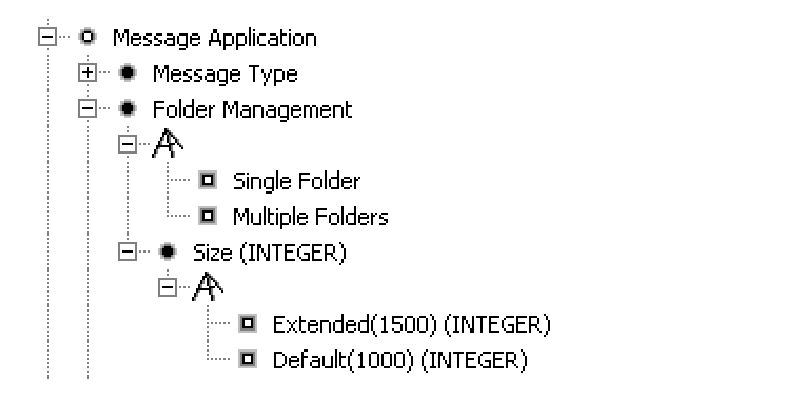
\includegraphics[scale=0.60]{img/fm03.eps}
%  \caption{Message Application feature model.}
%  \label{fig:fm-01}
%\end{figure}

%\begin{table}[h]
%\begin{tabular}{|l|l|}
%  \hline
%  {\bf Selected Feature} & {\bf Artifacts} \\ \hline \hline
%  Single Folder & Save Message (basic version) \\ \hline
%  Multiple Folders & Save Message (extended version) \\
%                   & Manage multiple folders use case \\
%  \hline
%\end{tabular}
%\caption{Folder management configuration.} \label{tab:ck-01}
%\end{table}

%Eriksson proposed the use of parameters in 
%order to describe crosscutting variabilities that change the behavior of different scenarios. 
%However, we believe that such kind of variability 
%should be described using quantification mechanisms, instead of parameters. In a previous work~\cite{gcabral-sbmf-2006}, the 
%quantification was achieved by enumerating all 
%the \emph{previous} and \emph{next steps} that delimits the starting and ending points of a given
%scenario (below we present our definition for scenario specification, 
%adapted from~\cite{gcabral-sbmf-2006}).

%\begin{description}
%\item[Scenario:] A use case scenario corresponds to a sequence of
%steps (a pair of \emph{User Action} x \emph{System Response}).
%Depending on the user action or system state, the behavior of a
%scenario can be changed. A use case defines a set of scenarios; and a use case model, 
%instead, defines a set of use cases.
%\end{description}

%In order to enable a better modularity (see figures~\ref{fig:pm-01} and~\ref{fig:alt-01}), a
%scenario could be \emph{started} from steps of different scenarios
%(using the \emph{from step} clause) and \emph{finished} by steps of
%other scenarios (using the \emph{to step} clause). Following the same 
%example of message application, two alternative flows are presented in Figure~\ref{fig:alt-01}. The first scenario,
%that allows a subscriber to save an edited message, changes the
%behavior of \emph{Create and Send a Message Scenario} (Figure~\ref{fig:pm-01})
%from \emph{Step 5M} to the \emph{end} of execution (see the
%\emph{from} and \emph{to step} clauses). The second one, instead, is
%an exception flow that describes the phone behavior when the
%subscriber tries to send or save a message and the message box is
%full. Such scenario changes the behavior of \emph{Create and Send a Message
%Scenario} (from \emph{Step 7M}) and \emph{Save a Message to Draft Folder Scenario}
%(from \emph{Step A1.1}). Such exception flow is an example of crosscutting
%variability, since it changes the behavior of multiple scenarios.

%Previously, only explicit references to the step ids (eg.: 5M, 7M,
%A1.1) are allowed in the \emph{from step} and \emph{to step}
%clauses~\cite{gcabral-sbmf-2006}. Therefore, the weaving rules of
%two or more scenarios are basically
%syntactic~\cite{rashid-aosd-2007}, resulting in \emph{fragile
%pointcuts} (a scenario composition could break, if we change a step
%id). In order to solve this problem, the use of semantic scenario
%compositions, based on the meaning of natural language
%specifications, was proposed by Rashid et
%al.~\cite{rashid-aosd-2007}. 

%In this paper, we propose a more simplistic semantic composition based on the use of annotations. We enrich scenario specifications 
%allowing a step to be marked with zero or more annotations; and the \emph{from steps} and \emph{to
%steps} clauses referring to steps in other scenarios by \emph{step ids}
%or by \emph{annotations}.

%
%\begin{figure}[h]
%%  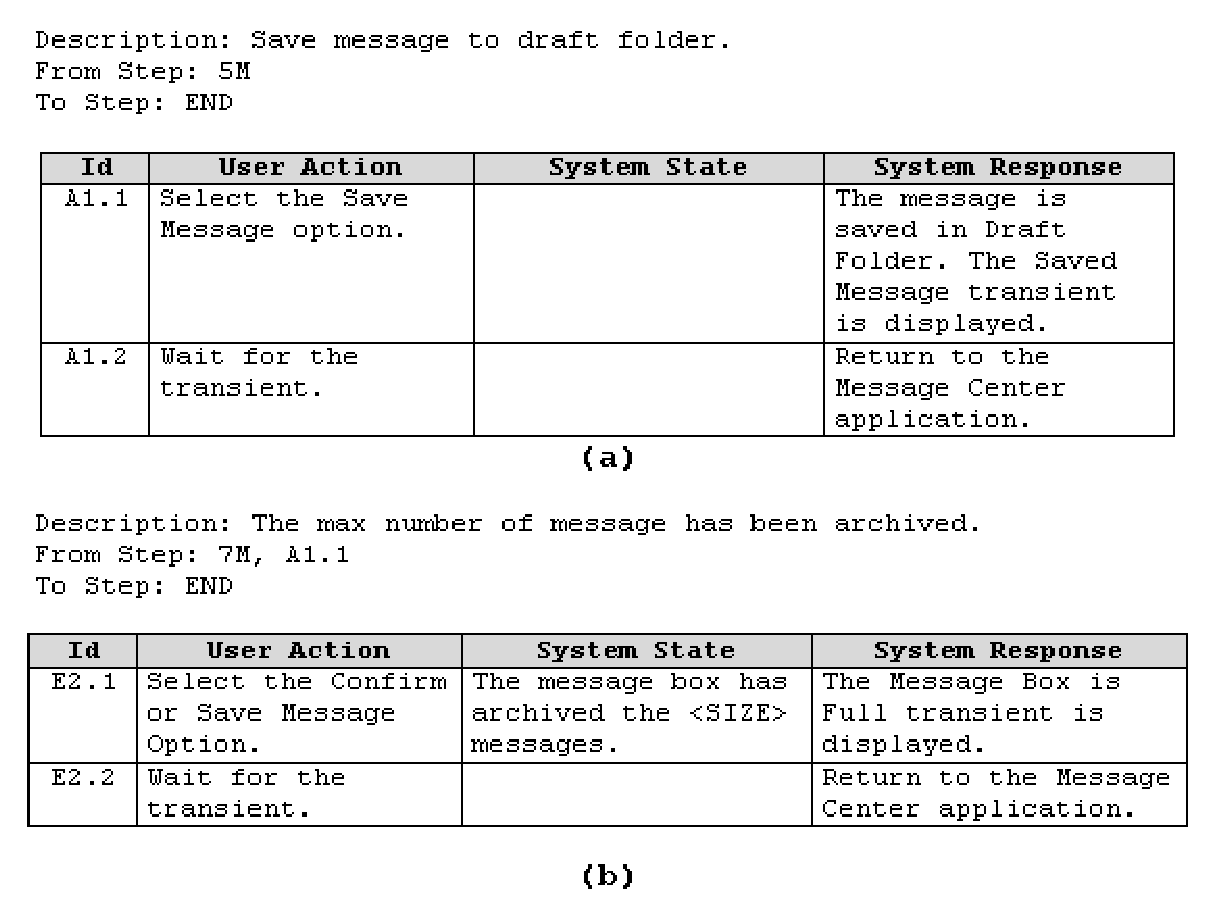
\includegraphics[scale=0.45]{img/alternative01.eps}
%  \begin{scriptsize} 
%  \texttt{
%  \begin{tabular}{l}
%  {\bf Basic Flow}\\
%  Description: Create and send a message.\\
%  From step: START\\
%  To Step: END\\
%  \end{tabular}  
%  \begin{tabular}{|p{0.2in}|p{0.8in}|p{0.8in}|p{1in}|}
%   \hline
%	Id & User Action & System State &  System Response \\ \hline \hline    
%	... & ... & ... & ... \\ \hline
%	3M  & Select a \mbox{<MessageType>} from the create message men.u & & The Create a New <MessageType> form is 
%displayed. \\ \hline
%	4M  & Fill the message body. & & The message body is filled. \\ \hline
%	5M  & Select the send message option. & The message body is not empty & The Recipient form is displayed. \\ \hline
%	6M  & Fill the recipient field. &  & The Recipient field is filled. \\ \hline
%	7M  & Select the confirm option. & The message box has not reached <Size> messages.  & The message is sent to the recipient 
%and saved in Sent Items folder. The Sent Message transient is displayed. \\ \hline 
%	... & ... & ... & ... \\ \hline
%  \end{tabular} 
%  }
%  \end{scriptsize}
%  \caption{Create and Send a Message scenario.}
%  \label{fig:pm-01}
%\end{figure}

%\begin{figure}[t]
%  \begin{scriptsize} 
%  \texttt{
%  \begin{tabular}{l}
%  Description: Save a message to draft folder\\
%  From step: 5M\\
%  To Step: END\\
%  \end{tabular}  
%  \begin{tabular}{|p{0.2in}|p{0.8in}|p{0.8in}|p{1in}|}
%   \hline
%	Id & User Action & System State &  System Response \\ \hline \hline    
%	A1.1 & Select the save message option. & There is enough space to save the message. &  The message is saved in draft folder. 
%The saved message transient is displayed. \\ \hline
%	A1.2 & Wait for the transient. & & Return to the Message Center Application.
%   \\ \hline
%  \end{tabular} 
%  }
%  \end{scriptsize}
%  \center{(a)}
%  
%  \begin{scriptsize} 
%  \texttt{
%  \begin{tabular}{l}
%  Description: The maximum number of messages has been achieved\\
%  From step: 7M, A1.1\\
%  To Step: END\\
%  \end{tabular}  
%  \begin{tabular}{|p{0.2in}|p{0.8in}|p{0.8in}|p{1in}|}
%   \hline
%	Id & User Action & System State &  System Response \\ \hline \hline    
%	E2.1 & Select the confirm or save message option. & Message box has achieved the <SIZE> messages. &  The Message Box is 
%Full transient is displayed. \\ \hline
%	E.2.2 & Wait for the transient. & & Return to the Message Center Application.
%   \\ \hline
%  \end{tabular} 
%  }
%  \end{scriptsize}
%  \center{(b)}
%  \caption{Send a Message alternative flows.}
%  \label{fig:alt-01}
%\end{figure}

%A final remark related to the scenario variability taxonomy is that we are proposing a new kind of variability: one that represents 
%parametric scenario specifications. Such kind of variability occurs whenever two similar behaviors vary only in accordance with 
%parameterized values. For example, Figure~\ref{fig:pm-01} depicts a scenario specification for \emph{sending a message} using 
%parameters  for reuse it with different \emph{kinds of message} (\emph{MessageType} parameter on step 3M) and \emph{message 
%folder sizes} (\emph{Size} parameter on step 7M). Parametric scenarios increase the requirement coverage and avoid duplicated 
%scenario specifications. Notice that the domain values for those parameters are defined in the feature model (features \emph
%{MessageType} and
%\emph{Size} in Figure~\ref{fig:fm-01}). In this way, the \emph{MessageType}
%parameter of step 3M abstracts over the different kinds of messages (\emph{email}, \emph{sms}, and \emph{mms}); and the  \emph
%{Size} parameter of step 7M abstracts over the values \emph{extended folder size} and \emph{default folder size} (Figure~\ref
%{fig:fm-01}).


%-------------------------------------------------------------------------
% Section: Modeling the Variability Mechanisms
%------------------------------------------------------------------------
\section{Variability as Crosscutting}
\label{sec:models}

Aiming to represent a clear separation between variability management and scenario specification, and also 
to describe the weave processes required to compose those views, we are proposing a modeling framework that is a 
customization of the Masuhara and Kiczales (MK) work~\cite{kiczales-ecoop-2003}. The goal of MK framework is to
explain how different \emph{aspect-oriented} technologies support crosscutting modularity. Each technology is modeled 
as a three-part description: the related weave processes take two programs as input, which crosscut each other with respect 
to the resulting program or computation~\cite{kiczales-ecoop-2003}. 

Similarly to the MK framework, we represent the semantics of \textbf{scenario variability management} as a weaver that takes four specifications
as input (\emph{product line use case model}, \emph{feature model}, \emph{product configuration}, and \emph{configuration knowledge}) that 
crosscut each other with respect to the resulting product specific use case model (Figure~\ref{fig:weave-process}). Combining these input languages, 
it is possible to represent the kinds of variability that we are interested in: \emph{optional use cases and scenarios}, \emph{quantified changed scenarios}, 
and \emph{parameterized} scenarios. 

A running example of our approach is presented in Section~\ref{sub:running}. After, we describe the semantics of our weaving process. For 
simplicity, it was decomposed in three subcomponents - one weaver process for each kind of variability.  The semantics of those 
weavers (and the meta-model of the input and output languages) are described using the Haskell programming language~\cite{haskell-report}. 
Such decision allows the execution and testing of concise weaving processes descriptions (all related source code is available at SPG web site~\cite{spg-url}) and keep our model close to MK work, which specifies their weaving processes using the Scheme programming language.

%\begin{figure}[h]
% 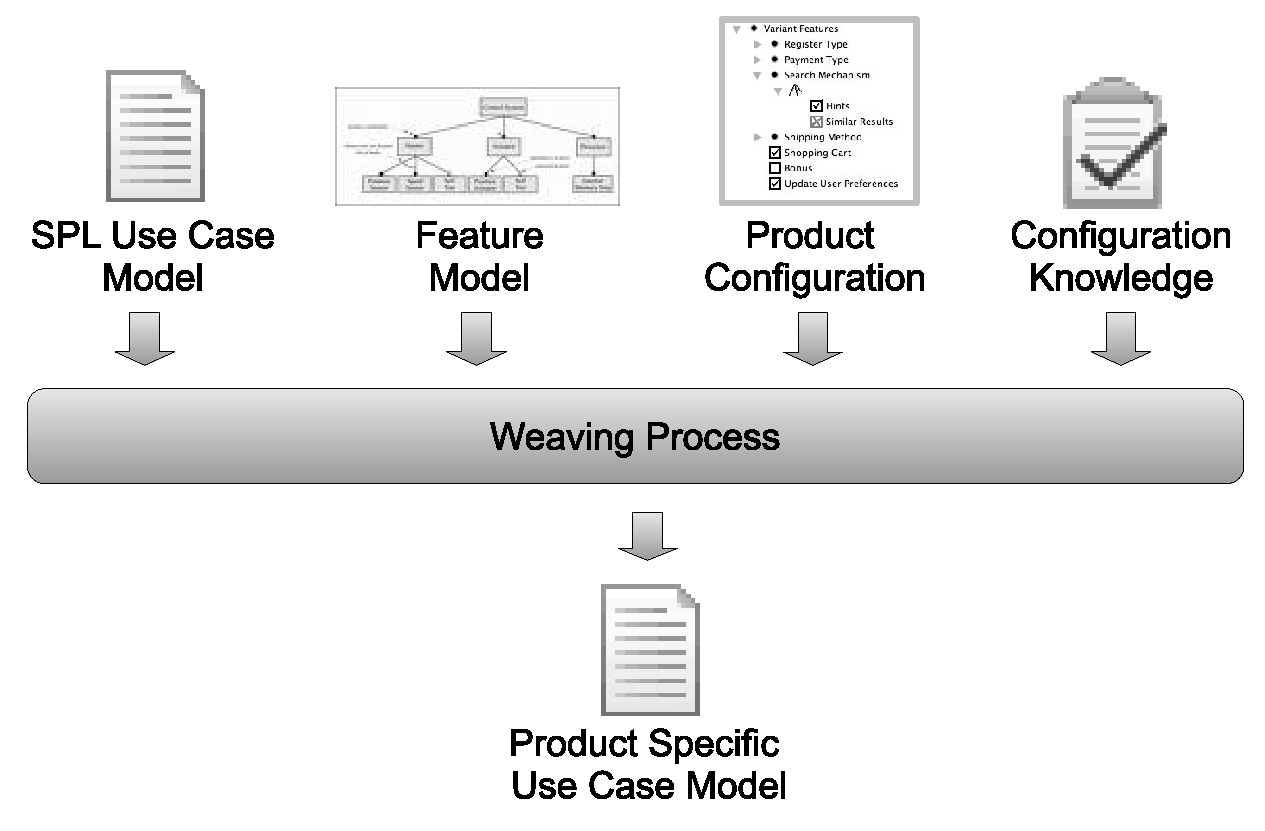
\epsfig{file=img/weave-process2.eps,scale=0.3}
% \caption{Overview of the modeling framework.}
% \label{fig:weave-process}
%\end{figure}

\begin{figure}[h]
 \begin{center}
  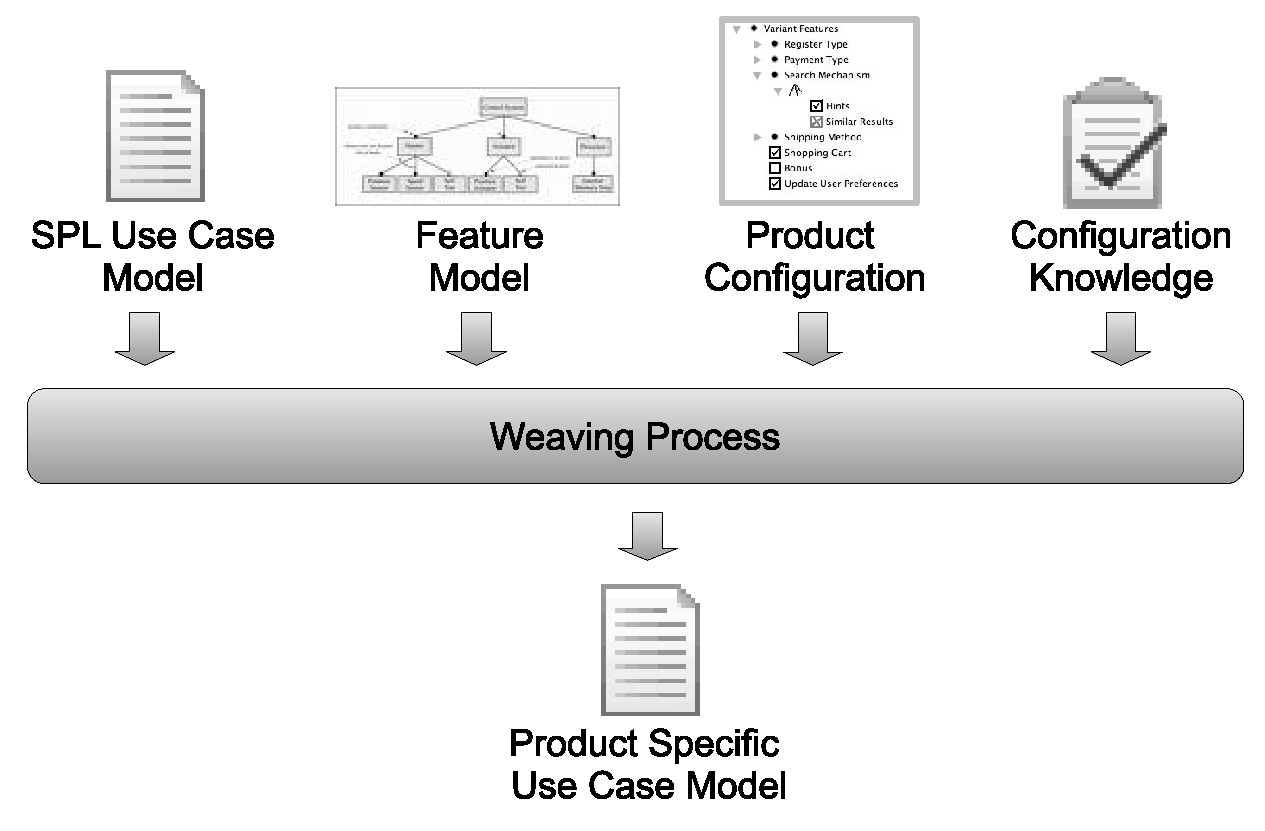
\includegraphics[scale=0.30]{img/weave-process2.eps}
  \caption{Overview of the modeling framework.}
  \label{fig:weave-process}
  \end{center}
\end{figure}

\subsection{Running example}
\label{sub:running}

In order to explain how the input languages crosscut each other and produce a product specific use case model, here we present a 
running example based on the eShop Product Line (briefly introduced in Section~\ref{sec:example}). For this, several artifacts of each 
input language are described. Then, we present the role of each input language in respect of the weaving process.


\subsubsection{SPL use case model}

This artifact defines a set of scenarios that might be used to describe possible variants of the product line. Although not being directly concerned 
with variability management, some scenarios might be optional, might have parameters, or might change the behavior of other 
scenarios. Based on the notation proposed in~\cite{gcabral-sbmf-2006},  a use case scenario corresponds to a sequence of
steps (a tuple of \emph{User Action} x \emph{System State} x \emph{System Response}).  A use case defines a set of scenarios; and a use case model, instead, defines a set of use cases. In this running example, we are considering the following scenarios:

{\bf Buy Products Basic Version:} this scenario (Figure~\ref{fig:buy-product-basic-flow}) specifies the basic behavior of \emph{Buy Products},
assembled in products that are not configured with the \emph{Shopping Cart} and \emph{Bonus} features. It starts from the IDLE special state 
(do not extend the behavior of an existing scenario) and finishes at the END of execution (in this case, there is no other behavior to be performed).
The clauses \emph{From step} and \emph{To step} are used for describing the possible starting and ending points of execution.
 
\begin{figure}[h]
\begin{scriptsize}
  \texttt{
   \begin{tabular}{l}
     Description: Basic version of Buy Products\\
     From step: IDLE \\
     To step: END
   \end{tabular}  
  \begin{center} 
  \begin{tabular}{|p{0.1in}|p{1.4in}|p{1.4in}|}
   \hline
       Id    & User Action  & System Response \\ \hline \hline
       1M & Select the buy product option.  & Present the selected product. The user can change the quantity of item that he wants to buy. Calculate and show the amount to be paid. \\  \hline
       2M & Select the confirm option. &  Request payment information. \\  \hline
       3M & Fill in the requested information and select the proceed option.  & Request the shipping method and address.\\  \hline
       4M & Select the <ShipMethod>, fill in the destination address and proceed. & Calculate the shipping costs. \\  \hline
       5M & Confirm the purchase. & Execute the order and send a request to the Delivery System to dispatch the products. 
       \mbox{[RegisterPreference]} \\  \hline
  \end{tabular}
  \end{center}
  } 
\end{scriptsize}
\caption{Basic version of Buy Products.}
\label{fig:buy-product-basic-flow}
\end{figure}

Notice that a parameter \emph{ShipMethod} is referenced in Step 4M of Figure~\ref{fig:buy-product-basic-flow}. The use of this parameter (notation also supported in PLUSS and PLUC) allows the reuse of this specification 
for different kinds of \emph{ship method} configurations.

{\bf Buy Products with Shopping Cart and Bonus:} this scenario (Figure~\ref{fig:buy-product-changing-flow}) changes the behavior of the \emph{Buy Products Basic Version} by replacing its first two steps and by introducing the specific behavior required by the \emph{Shopping Cart} and 
\emph{Bonus} features. This scenario starts from the IDLE state (\emph{from step} clause) and returns to the third step of the \emph{Buy Products Basic Version} (\emph{to step} clause). This behavior is required for products that are configured with \emph{Shopping Cart} and \emph{Bonus} features.

\begin{figure}[h]
\begin{scriptsize}
  \texttt{
   \begin{tabular}{l}
     Description: Extended version of Buy Products\\
     From step: IDLE \\
     To step: 3M
   \end{tabular}  
  \begin{center} 
   \begin{tabular}{|p{0.1in}|p{1.4in}|p{1.4in}|}
   \hline
       Id & User Action & System Response \\ \hline \hline
       V1 & Select the checkout option.  & Present the items in the shopping cart and the amount to be paid. The user can remove items from shopping cart. \\  \hline
       V2 & Select the confirm option. & Request bonus and payment information. \\  \hline
  \end{tabular}
  \end{center}
  } 
\end{scriptsize}
\caption{Extended version of Buy Products.}
\label{fig:buy-product-changing-flow}
\end{figure}

{\bf Search for Products:} this scenario allows the user to search for products. In order to save space, we are only presenting the Step 3S, which performs a search based on the input criteria (Figure~\ref{fig:search-products-flow}). This step is annotated with the mark \mbox{{\bf [RegisterPreference]}}, exposing it as a possible point that the behavior of \emph{Register User Preferences} might starts. The same annotation was used in the Step 5M of \emph{Buy Products Basic Version}. Such annotations can be referenced in the \emph{from step} and \emph{to step} clauses, reducing the problem of \emph{fragile pointcuts}~\cite{rashid-aosd-2007}.

\begin{figure}[t]
\begin{scriptsize}
  \texttt{
   \begin{tabular}{l}
     Description: Search for Products scenario\\
     From step: IDLE \\
     To step: END
   \end{tabular}  
  \begin{center} 
   \begin{tabular}{|p{0.1in}|p{1.4in}|p{1.4in}|}
   \hline
       Id & User Action &  System Response \\ \hline \hline
       \ldots & \ldots  & \ldots \\  \hline
       3S & Inform the search criteria. &  Retrieve the products that satisfy the search criteria. Show a list with the resulting products. [RegisterPreference] \\  \hline
  \end{tabular}
  \end{center}
  } 
\end{scriptsize}
\caption{Search for Products scenario.}
\label{fig:search-products-flow}
\end{figure}

{\bf Register User Preferences:} this scenario updates the user preferences based on the buy and search products use cases. Its behavior can be 
started at each step that is marked with the {\bf [RegisterPreference]} (see the \emph{from step} clause) annotation and is available in products 
that are configured with the \emph{Register User Preferences} feature.

\begin{figure}[h]
\begin{scriptsize}
  \texttt{
   \begin{tabular}{l}
     Description: Register user preferences.\\
     From step: [RegisterPreference] \\
     To step: END
   \end{tabular}  
  \begin{center} 
   \begin{tabular}{|p{0.1in}|p{1.4in}|p{1.4in}|}
   \hline
       Id & User Action &  System Response \\ \hline \hline
       1R & - &  Update the preferences based on the search results or purchased items. \\  \hline
  \end{tabular}
  \end{center}
  } 
\end{scriptsize}
\caption{Register user preferences.}
\label{fig:register-preferences-flow}
\end{figure}

\subsubsection{Feature model}

We have introduced part of this artifact for the eShop product line in Section~\ref{sec:example}. However, here we are going to 
present only the features required  (Figure~\ref{fig:eshop-fm-re}) for understanding the running example. 

 \begin{figure}[h]
 \begin{center}
  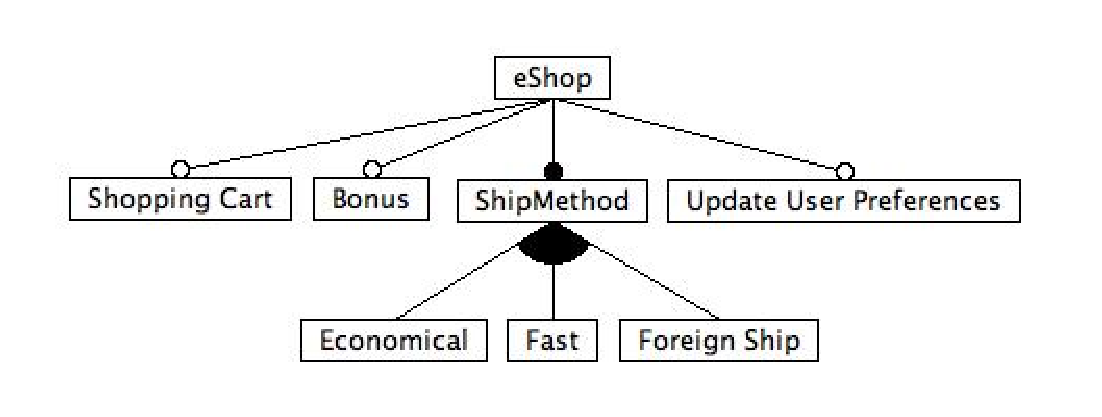
\includegraphics[scale=0.40]{img/eShop-fm-re.eps}
   \caption{Subset of eShop feature model.}
  \label{fig:eshop-fm-re}
  \end{center}
\end{figure}

Based on the feature model of Figure~\ref{fig:eshop-fm-re}, the \emph{Shopping 
Cart}, \emph{Bonus} and \emph{Update User Preferences} features are not required; on the other hand, the feature \emph{Ship Method} is mandatory and all specific products might be configured with at least one of its child.  

\subsubsection{Product configuration}

This artifact is used for identifying which features were selected in order to compose a specific member of a product line. Each product configuration should be conform to a feature model (the selected features should obeyed the feature model relationships and constraints). Two possible configurations are presented in Figure~\ref{fig:product-config-01-02}.  

\begin{figure}[t]
  \centerline{
    \mbox{
\includegraphics[scale=0.4]{img/pc-01.eps}}
    \mbox{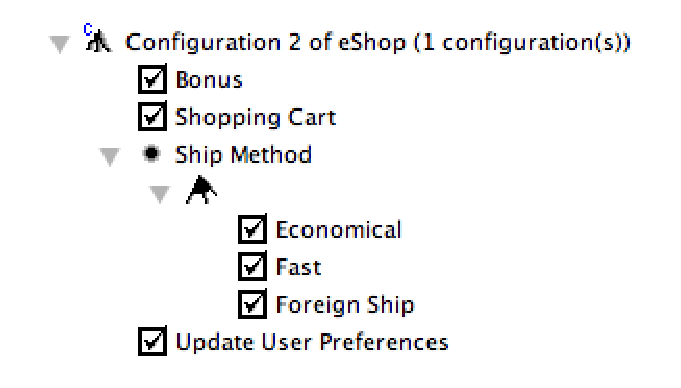
\includegraphics[scale=0.4]{img/pc-02.eps}}
  }
  \caption{Examples of product configurations.}
  \label{fig:product-config-01-02}
  \end{figure}
  
The first configuration (on the left side of the Fgure~\ref{fig:product-config-01-02}) defines a product that has no support for shopping cart, bonus and preferences update. Additionally, it supports only the economical and fast ship methods. The second configuration selects all possible features. 

\subsubsection{Configuration knowledge}

This artifact is used for relating feature expressions to artifacts that must be assembled in a given product. Such artifact allows, during the product engineering phase, the automatic selection of assets that are required for a specific product configuration. Table~\ref{tab:eshop-running-example} presents a configuration knowledge 
for the running example, enforcing that: if \emph{Shopping Cart} and \emph{Bonus} features are {\bf not} selected, the 
basic version of \emph{Buy Product} scenario will be assembled; otherwise, the extended version of the same 
scenario will be assembled; and the \emph{Register User Preferences} scenario will be assembled only if the \emph{Update 
User Preferences} feature is selected.

\begin{table}[h]
\begin{center}
\caption{eShop configuration knowledge} \label{tab:eshop-running-example}
\begin{tabular}{ll}
   \hline\noalign{\smallskip}
  {\bf Expression} & {\bf Required Artifacts} \\
   \noalign{\smallskip}
   \hline
   \noalign{\smallskip}
    \ldots & \ldots \\
    {\bf not} (Cart {\bf and} Bonus)\hspace{2pt} & Basic version of Buy Products \\
    Cart {\bf and} Bonus & Extended version of Buy Products \\
    Update Preferences & Register user preferences	 \\       
  \hline
\end{tabular}
\end{center}
\end{table}


\subsubsection{Weaving process}

After presenting input artifacts for the running example, we are ready to describe the weaving process that combine 
the input languages in order to manage scenario variabilities. In the next section we present, more precisely, the semantics of its components using a low level design. The weaving process is composed by four activities, although the last one is optional:

{\bf Validation activity:} This activity is responsible for checking if a product configuration is a valid instance of the feature model. If the product configuration is 
valid (it is conform to the relationship cardinalities and constraints of the feature model), the process might proceed. Otherwise, an error should be reported. 

{\bf Product derivation activity:} This activity takes as input a (valid) product configuration and a configuration knowledge. 
Then, each feature expression of the configuration knowledge is checked against the product configuration. If the expression 
is satisfied, the related scenarios are assembled as the result of this activity. For the running example, 
Table~\ref{tab:assembled-scenarios} shows the assembled scenarios for the configurations depicted in Figure~\ref{fig:product-config-01-02}.

\begin{table}[h]
\begin{center}
\caption{Assembled scenarios} \label{tab:assembled-scenarios}
\begin{tabular}{ll}
   \hline\noalign{\smallskip}
  {\bf Configuration} & {\bf Assembled scenarios} \\
   \noalign{\smallskip}
   \hline
   \noalign{\smallskip}
    Configuration 1\hspace{15pt} & Basic version of Buy Products \\
                             & Search for products \\
                             & \ldots \\
   Configuration 2 & Extended version of Buy Products \\
                             & Search for Products	 \\
                             & Register user Preferences \\
                             & \ldots       \\
  \hline
\end{tabular}
\end{center}
\end{table}
 
 {\bf Scenario composition activity:} This activity is responsible for composing the scenarios assembled for a specific product configuration. 
 The resulting scenarios of the previous activity, which crosscut each other based on the \emph{from step} and \emph{to step clauses}, are woven. The 
 result is either a use case model with complete paths (all \emph{from step} and \emph{to step} clauses are resolved) or a trace model (a set of all valid sequences of events extracted from the complete paths). 
 
The complete path is a high level representation, which uses the same constructions of the use case model (scenarios), and can be better understood using a graph notation, where each node is labeled with a step id. For example, Figure~\ref{fig:complete-paths} depicts the complete paths for the first and second configurations of our running example. In the left side of the figure,  the basic versions of search for product (branch labeled as 1S, 2S, 3S) and buy product (branch labeled as 1M, 2M, ..., 5M) scenarios are presented. Instead, on the right side of the figure, the extended versions of these scenarios are presented. In this case, steps 1M and 2M have been replaced by steps V1 and V2 (because \emph{Shopping Cart} and \emph{Bonus} features are selected) and the step  1R is introduced after steps 5M and 3S (because \emph{Update User Preferences} is selected in this configuration).
 
Instead, the trace model can be seen as a low level representation of the use case model. Such notation has a well defined semantic and might 
be used for model checking and test case generation. Such applications of the trace model are beyond the scope of this paper. More information 
can be found elsewhere\cite{csp-hoare,csp-roscoe,cfeitosa-sbmf-2006}. Here, the trace model is useful for implementing the last activity of our weave process, binding parameters, and 
represents all possible sequences of events in a specific product configuration. 


 
\begin{figure}[t]
\begin{center}
\begin{tiny}
\begin{xy}
\xymatrix@R=10pt{
& *++[o][F-]{idle} \ar[r]\ar[d] & *++[o][F-]{1M} \ar[d]	& *++[o][F-]{idle} \ar[r]\ar[d] & *++[o][F-]{V1} \ar[d] 	\\
& *++[o][F-]{1S} \ar[d]  & *++[o][F-]{2M} \ar[d]           & *++[o][F-]{1S} \ar[d]  & *++[o][F-]{V2} \ar[d] 			\\
& *++[o][F-]{2S} \ar[d]  & *++[o][F-]{3M} \ar[d]           & *++[o][F-]{2S} \ar[d]  & *++[o][F-]{3M} \ar[d]			\\
& *++[o][F-]{3S} \ar[d]  & *++[o][F-]{4M} \ar[d]           & *++[o][F-]{3S} \ar[d]  & *++[o][F-]{4M} \ar[d] 			\\
& *++[o][F-]{end} & *++[o][F-]{5M} \ar[l]                     & *++[o][F-]{1R} \ar[d] & *++[o][F-]{5M} \ar[l]   			\\
&                         &                                                    &   *++[o][F-]{end}       &
}
\end{xy}
\end{tiny}
\caption{Complete paths represented  as a graph}
\label{fig:complete-paths}
\end{center}
\end{figure}

For instance, the trace model for the first configuration is the set of sequences:

\begin{small}
\begin{tabular}{rlc}
$Trace_{C1}$ = & \{<>, <idle>, <idle, 1S>, <idle, 1S, 2S>, \\ 
                    & <idle, 1S, 2S, 3S>,  <idle, 1S, 2S, 3S, end>, \\ 
                    & <idle, 1M>, <idle, 1M, 2M>, \ldots, \\ 
                    & <idle, 1M, 2M, 3M, 4M.ShipMethod, 5M, end> \}
\end{tabular}
\end{small}
 
{\bf Binding parameters activity:}  This optional activity takes as input the assembled scenarios and the product configuration and generates 
 a trace model resolving all parameters referenced by the steps. For example, step 4M in Figure~\ref{fig:buy-product-basic-flow} has a reference 
 to the parameter \emph{ShipMethod}. The parameter values are defined in the product configuration.
 
For instance, in the first configuration depicted in Figure~\ref{fig:product-config-01-02}, the parameter \emph{ShipMethod} might assume the values \emph{Economical} or \emph{Fast}. In order to reduce the coupling between scenario specifications and feature model, a mapping (or environment) is used for relating scenario parameters to features. For each trace that contains a parameterized event (or step), this activity creates a new trace for all of the possible parameter values. Consequently, resolving parameters for the trace $<idle,1M,2M,3M,4M.ShipMethod>$ results in the following sequences:
 
\begin{center} 
\begin{small}
\begin{tabular}{c}
<idle,1M,2M,3M,4M.Economical>, \\ <idle,1M,2M,3M,4M.Fast>, \\
\end{tabular}
\end{small}
\end{center}

Next, we introduce the modeling framework used to formally describe the composition processes introduced in this running example. 


\subsection{Modeling Framework}

As presented before, we are proposing, based on the Masuhara and Kiczales work~\cite{kiczales-ecoop-2003}, a crosscutting 
variability management approach. Their requirement for characterizing a mechanism as crosscutting is fulfilled by our approach, since different specifications contribute to the definition of a specific SPL member. Additionally, due to its crosscutting nature, the modeling framework proposed in~\cite{kiczales-ecoop-2003}  is suitable for formalizing variability management compositions. 
Our weaving process is modularized in three major components, formally described in sections~\ref{sub:pd-weaver}, \ref{sub:sc-weaver}, \ref{sub:bind-weaver}. Actually, each of this components is also a weaver. As a customization of MK work, our modeling framework, used to describe these weavers, is an 7-tuple (Eq.~\ref{eq:tuple} and Table~\ref{tab:tup-01}) that highlights the importance of the composition process languages. 

\begin{equation}
T = \{o, o_{jp}, L, L_{id}, L_{eff}, L_{mod}, meta\}, where:
\label{eq:tuple}
\end{equation}

\begin{table}[h]
\begin{center}
\caption{Modeling framework elements.} \label{tab:tup-01}
\begin{tabular}{|p{0.6in}|p{2.4in}|}
  \hline
  {\bf Element} & {\bf Description} \\ 
   \hline
  $o$              & Output language used for describing the results of the weave process \\ \hline
  $o_{jp}$       & Set of join points in the output language \\ \hline
  $L$              & Set of languages used for describing the input specifications \\ \hline
  $L_{ID}$      & Constructions in each input language used for identifying the output join points \\ \hline 
  $L_{EFF}$   & Effect of $l'$ constructions in the weaving process, where $l \in L$ \\ \hline
  $L_{MOD}$  & Modular unities of each input language \\ \hline
  $meta$         & An optional argument used for customizing the weave process \\ 
  \hline
\end{tabular}
\end{center}
\end{table}

Each component is responsible for realizing one variability mechanism. We represent them by 
filling in the seven parameters of our modeling framework and by stating 
how elements of the weaver implementation correspond to elements of the model.

% ---
% Product derivation weaver
% ---
\subsubsection{Product derivation weaver}\label{sub:pd-weaver}

This weaver is responsible for selecting artifacts based on specific product configurations. 
As a consequence, it is worried about the first two activities of our variability management approach: 
validating a product configuration against  a feature model and selecting a subset of the SPL assets. 
In this paper, we focus only in the selection of scenarios that should be assembled in specific instances 
of the SPL. However, this weaver often is required for managing variabilities in other kinds of artifacts.  
For instance, applying this weaver for combining the eShop use case model, feature model , and configuration knowledge with the configuration depicted in right side of Figure~\ref{fig:product-config-01-02} will result, beside others, in the selection of the extended version of \emph{Buy Products} scenario (Figure~\ref{fig:buy-product-changing-flow}).  
 
This weaver, implemented by the function \emph{pdWeaver} (Listing~\ref{lst:configure}), takes as input 
a \emph{SPL use case model} (UCM), a \emph{feature model} (FM), a \emph{product configuration} (PC), and a \emph{configuration knowledge} (CK). Initially, this function verifies if the product configuration is a well formed instance of the feature model (\emph{validInstance} function) - if it is not the case,  an \emph{InvalidProduct} error is thrown. Then, the IDs of required scenarios are computed by the \emph{configure} function. This is done by evaluating which feature expressions (list \emph{x:xs}), in the configuration knowledge, are valid for the specific instance (\emph{eval} function). Finally, given the resulting list of scenario IDs, 
the function \emph{retrieveArtifacts} returns the product specific scenarios.

The model of \emph{Product Derivation Weaver}, 
in terms of the framework, is showed in Table~\ref{tab:pd-weaver}. The \emph{pdWeaver} function is used to argue that the model is realizable and appropriate~\cite{kiczales-ecoop-2003}. We achieve this by matching the model elements 
to corresponding parameters and auxiliary functions in the implementation code. Therefore, the input languages UCM, FM, CK, and PC are represented as different parameters 
of the \emph{pdWeaver} function. An instance of the UCM corresponds to the specification of all 
SPL scenarios. A FM instance is only responsible for declaring the SPL features and the relationships between 
them; as a consequence, there is no coupling between FMs and UCMs. Instead, relationships between features and artifacts are documented in the configuration knowledge. Finally, the PC specifies which features were selected 
for a specific product. 

\begin{lstlisting}[belowskip=20pt,frame=tb,caption={The \emph{configure weaver} function},label=lst:configure]
pdWeaver :: UCM -> FM -> PC -> CK -> ScenarioList
pdWeaver ucm fm pc ck = 
 if not (validInstance fm pc) 
 then error InvalidProduct
 else retrieveScenarios ucm (configure pc ck)

configure :: PC -> CK -> ArtifactIdList
configure pc (CK []) = []
configure pc (CK (x:xs)) =
 if (eval pc (expression x))
  then (artifacts x) ++ (configure pc (CK xs))
  else configure pc (CK xs)
\end{lstlisting}


The UCM has a greater importance over the other input languages ($UCM_{EFF}$), since it declares the product specific scenarios (the 
output of this weaver process generated by the \emph{pdWeaver} function). These scenarios ($UCM_{ID}$) are used in the \emph{retriveScenarios} function in order to identify which artifacts will be assembled in the final product.     

In order to identify which artifacts are required for a specific product, the \emph{configure} function ($CK_{EFF}$) checks the feature expression ($CK_{ID}$) against the product specific features ($PC_{ID}$). The effect of FM in this weaver ($FM_{EFF}$) is to check if the PC is well formed. Such evaluation is implemented by the \emph{validInstance} function and considers the PC feature selection ($PC_{EFF}$). 

The product derivation weaver is not parameterized. So, the \emph{meta} element of the modeling framework is not considered in this case.   

\begin{table}[bh]
\begin{center}
\caption{Model of Product Derivation} \label{tab:pd-weaver}
\begin{tabular}{p{0.6in}p{2.4in}}
   \hline\noalign{\smallskip}
  {\bf Element} & {\bf Description} \\
   \noalign{\smallskip}
   \hline
   \noalign{\smallskip}
   $o$               & Product specific scenarios (list of scenarios) \\ 
   $o_{jp}$        & Scenario declarations \\ 
   $L$               & \{UCM, FM, CK, PC\} \\ 
   $UCM_{ID}$ & SPL scenarios \\ 
   $FM_{ID}$    & SPL features \\ 
   $CK_{ID}$    & Feature expressions \\  
   $PC_{ID}$    & Product specific feature selection \\ 
   $UCM_{EFF}$ & Provides declaration of scenarios \\  
   $FM_{EFF}$    & Checks if a SPL instance is well formed \\ 
   $CK_{EFF}$    & Defines the required artifacts  \\ 
   $PC_{EFF}$    & Specifies the configuration of a product \\
   $UCM_{MOD}$ & Scenario \\  
   $FM_{MOD}$   & Feature \\ 
   $CK_{MOD}$    & Each pair $(feature\ expression, artifact\ list)$  \\ 
   $PC_{MOD}$    & Feature \\
   $meta$         & - \\ 
  \hline
  \end{tabular}
\end{center}
\end{table}



% ---
% Scenario composition weaver
% ---

\subsubsection{Scenario composition weaver}\label{sub:sc-weaver}

This weaver is responsible for the third activity of our variability management 
approach. It aims at composing variant scenarios of a use case~\cite{gcabral-sbmf-2006} and 
is applied whenever a use case scenario supports different paths of execution, based on the product configuration.
This mechanism takes as input the product specific use case model (a list of scenarios). Each flow of events 
(usually a partial specification) must be composed in order to generate a concrete scenario.

A variant scenario 
might refer to steps either in basic or other alternative scenarios. In order
to compute the complete paths defined by a scenario, we need to compose,
recursively, the events that precede all of the steps referenced by its \emph{from step
clause} (until the IDLE state), plus its own steps, plus all the
events that follow all of the steps referenced by its \emph{to step clause} (until the END
state)\footnote{IDLE and END states are predefined steps that
represent the \emph{beginning} and the \emph{end points} of a
specification.}. 

For instance, consider a product configured with the features \emph{Shopping Cart} and \emph{Bonus}, which requires the extended version of \emph{Buy Product} scenario, and with the feature \emph{Update User Preferecens}. Referring to Figure~\ref{fig:buy-product-changing-flow}, the extended version of 
\emph{Buy Product} scenario starts from the IDLE state (\emph{from step} clause) and then, after its own flow of events, goes back to Step 3M of \emph{Buy Product} basic version (\emph{to step} clause). In a similar way, Figure~\ref{fig:register-preferences-flow} depicts that \emph{Register User Preferences} scenario starts from any step that is marked with the \emph{RegisterPreferences} annotation (for example, Step 5M of the basic version of \emph{Buy Product}). In this context, the result of applying the composition scenario weaver is a concrete path of execution for this configuration, that can be represented as the sequence of step ids: 

\begin{center}
\mbox{<IDLE, V1, V2, 3M, 4M.ShipMethod, 5M, 1R, END>}.
\end{center}

Note that this sequence still has  the \emph{ShipMethod} parameter, 
referred in Step 4M of \emph{Buy Product} basic flow. Listing~\ref{lst:ucm} presents the 
abstract representation of the use case model, use case, and scenario artifacts. 
Some elements of the abstract syntax, which are not required for understanding this weaver, 
are not presented in Listing~\ref{lst:ucm}. Briefly, a use case model has a name and a list of use cases. 
A use case has an id, a name, a description, and a list of scenarios (that defines its
basic, alternative, and exception flows). A scenario has an id, a
description, a \emph{from step clause} (a list of references for
existing steps), a list of steps, and a \emph{to step clause} (also
a list of references for existing steps). A step has an id, a
a specification in the form of a tuple
(user-action x system-state x sytem-response), and a list of annotations
that can be used to semantically identify the step (avoiding
the problem of fragile pointcuts). Finally, a reference to a step can be either a reference to a \emph{step id} or to a \emph{step annotation}.

\begin{lstlisting}[belowskip=10pt,frame=tb,caption={Use Case abstract syntax},label=lst:ucm]
data UseCaseModel = UseCaseModel Name UseCaseList
data UseCase = UseCase Id Name ScenarioList
data Scenario = Scenario Id FromStep StepList ToStep
data Step = Step Id Action State Response Annotations
\end{lstlisting}

The \emph{Scenario Composition Weaver} is implemented by the \emph{scWeaver} function (Listing~\ref{lst:trace}), which takes 
as input the SPL use case model and a product specific list of scenarios (that may be computed by the previous weaver). The SPL 
use case model is required in this composition because a product specific scenario is able to refer to a step that is defined in the 
SPL scenarios but was not selected in a specific configuration. 
 
This implementation computes the complete paths of each product specific 
scenario by calling, recursively, the \emph{completePaths} function. This 
function (lines 5-7 in Listing~\ref{lst:trace}) 
takes as input the whole use case model (\emph{ucm}) and a scenario (\emph{scn});
and returns all complete paths (a list of \emph{step lists}) of
\emph{scn}. The function \emph{fromList} (called at line 7) is used to
compose all complete paths extracted from the \emph{from step
clause}. In a similar way, the function \emph{toList} (called at
line 7) is used to compose all complete paths extracted from the
\emph{to step clause}. The \emph{match} function (also called at
line 7), retrieves all the steps in \emph{ucm} that satisfy all 
\emph{step references} in \emph{from step} or \emph{to step}
clauses. Currently, this matching is based on the \emph{step id} (a
syntactically reference) or on the list of \emph{step annotations}
(a semantic reference). The ``+++'' operator denotes a distributed
list concatenation.

After computing the complete paths, it is possible to derive a reasonable representation 
for the product specific scenarios. We named this representation as \emph{trace model}, since 
it describe all possible sequences of events produced by the complete paths. This representation is 
useful for checking, for example, if a non-expected sequence of events is present in a final product, which 
means that a problem in the composition process has occurred. The \emph{traceModel} 
function (lines 9 and 10 of Listing~\ref{lst:trace}) is responsible for computing this representation. 
Such function takes as argument another function \emph{f} and a list of steps (\emph{x:xs}).
Currently, the valid functions that can be applied as the first argument are the \emph{stepId} function (returns the id
of a given step) and the \emph{bind e} function (that also computes the
parameter values of a given \emph{step} in a specific \emph{feature
environment}). Therefore, if we are interested in the trace model representation, the \emph{Scenario 
Composition Weaver} can be configured (the \emph{META} element of
our modeling framework) to return:  a) a trace model without parameters, computed
for each complete path of the resulting scenarios; or b) a trace model,
with resolved parameters, for each complete path of the resulting scenarios.  Next section we explain 
the \emph{bind} and \emph{feature environment} constructions. 

The model of this weaver is depicted in Table~\ref{tab:sc-weaver}. 

\begin{table}[bh]
\begin{center}
\caption{Model of Scenario Composition Weaver} \label{tab:sc-weaver}
\begin{tabular}{p{0.6in}p{2.4in}}
   \hline\noalign{\smallskip}
  {\bf Element} & {\bf Description} \\
   \noalign{\smallskip}
   \hline
   \noalign{\smallskip}
   $o$               & List of concrete scenarios or trace models  \\ 
   $o_{jp}$        & Scenarios and steps of scenarios \\ 
   $L$               & \{use cases and scenarios\} \\ 
   $L_{ID}$       & From step and to step clauses \\ 
   $L_{EFF}$    & Compose concrete scenarios  \\ 
   $L_{MOD}$ & Use cases and scenarios \\  
   $meta$          & Function used to parameterize the trace model generation \\ 
  \hline
  \end{tabular}
\end{center}
\end{table}


\begin{figure*}
\begin{lstlisting}[belowskip=10pt,frame=tb,caption={The \emph{completePaths} and \emph{traceModel weaver} 
functions},label=lst:trace]
scWeaver :: UseCaseModel -> ScenarioList -> [StepList]
scWeaver ucm [] = []
scWeaver ucm (x:xs) = (completePaths ucm x) ++ (scWeaver ucm xs)
 
completePaths :: UseCaseModel -> Scenario -> [StepList]
completePaths ucm scn =
 (fromList ucm (match ucm (fromStepsOf scn)) +++ [stepsOf scn]) +++  (toList ucm (match ucm (toStepsOf scn)))

traceModel f [] = [[]]
traceModel f (x:xs) = [] : (f x) ^ (traceModel f (xs))
\end{lstlisting}
\end{figure*}

The output ($o$ element of our modeling framework) can be either the concrete product specific scenarios, 
computed directly from \emph{scWeaver} function; or a trace model, computed by calling the \emph{traceModel} function for each 
concrete scenario. The input languages (L) are both the SPL use case model and the product specific scenarios. These (similar) input languages 
correspond to the parameters of \emph{scWeaver} function. 

The join points are modeled as the final scenarios and steps in the output language. They result from the composition of partial scenarios by means of 
\emph{from steps} and \emph{to steps} clauses ($L_{ID}$).  The effect of the input languages ($L_{EFF}$) in the composition process is to combine 
product specific scenarios that, before this activity, should not define a concrete flow of events. As a consequence, the \emph{match} function 
plays a fundamental role in this process, retrieving the steps in the use case model that satisfies the \emph{from step} and \emph{to step} clauses.  
 Finally, as we have explained before, such mechanism is
parameterized (the $META$ element of our customized framework) in
order to select, once the trace model was selected as the output language,  if the parameters will be resolved 
or not.


% ---
% Bind parameters weaver
% ---

\subsubsection{Bind parameters weaver}\label{sub:bind-weaver}

This weaver is responsible for the third activity of our variability
management approach. Parameters are used in scenario specifications 
in order to create reusable requirements. This kind of variability can be applied
whenever two or more scenarios share the same behavior (the sequence
of actions) and differ in relation only to values of a same concept.
For instance, Figure~\ref{fig:buy-product-basic-flow} depicts the \emph{Buy Products} 
scenario that can be reused for different \emph{ship methods}. Without this
parameterized specification, and aiming at automatically generating, for example, a test case suite 
with a good coverage, it would be necessary to create a specification for each kind of ship method.

This weaver takes in consideration \emph{scenario specifications} and 
\emph{product configurations}, which defines the domain values of a
parameter. Thus, in order to reduce the coupling between scenarios and features, 
we are proposing an environment that relates them. Features related to parameters must be 
either an {\bf alternative feature} or an {\bf or feature}~\cite{gheyi-alloy-06,czarnecki-wsfactory-2005,czarnecki-book}.

The implementation of this weaver consists in a call to 
the \emph{traceModel} function (Listing~\ref{lst:trace}) with
the \emph{bind e} partial function as first parameter. The
\emph{bind} function (lines 1-5 of Listing~\ref{lst:bind}) takes as
input an environment (\emph{e}), that maps a parameter into a
feature, and a step (\emph{s}). Then, it extracts all parameters
from \emph{s}, and returns a suitable event representation with the
corresponding parameter values. Each text between the symbols ``$<$'' and ``$>$''
(defined in the user action, system state, or system response of a
step) is treated as a parameter and must be defined in the
environment (otherwise, an type exception is thrown).

For example, if a product is configured with either \emph{Fast} and 
\emph{Economical} ship methods, the result of applying this weaver for 
the Step 4M of the Buy Product basic version will result in the following 
representation: 4M(Fast, Economical)  

The \emph{extractParameterValues} function (called at line 5 of
Listing~\ref{lst:bind}) is responsible for extracting the related
parameter values from a feature. Also, each parameter must be
related to an {\bf alternative feature} or to an {\bf or feature}
present in a product configuration. 

\begin{lstlisting}[belowskip=10pt,frame=tb,caption={The \emph{bind weaver} function},label=lst:bind]
bind :: Environment Feature -> Step -> Event
bind e x =
 if (length (extractParameters (details x)) == 0)
  then stepId x
  else stepId x ++ (extractParameterValues e x)
\end{lstlisting}

The description of the Bind Parameters model is 
showed in Table~\ref{tab:bp-weaver}. This weaver just resolve parameters in 
the trace model representation. Therefore, its output language is also the set 
of all valid sequences of events (a trace model) with binding parameters (join points). 
The use case model (UCM) defines the list of scenarios that might be parameterized ($UCM_{EFF}$). Each scenario 
parameter ($UCM_{ID}$), indeed, contributes to the definition of one join point in this weaver. The 
other contributions come from the configuration knowledge (CK), in the sense that the domain values 
of a parameter is defined ($CK_{EFF}$) in the product specific features. The environment ($e$ parameter of the \emph{bind} function) is 
used for relating parameters to features. 

\begin{table}[h]
\begin{center}
\caption{Model of Bind Parameters Weaver} \label{tab:bp-weaver}
\begin{tabular}{p{0.6in}p{2.4in}}
   \hline\noalign{\smallskip}
  {\bf Element} & {\bf Description} \\
   \noalign{\smallskip}
   \hline
   \noalign{\smallskip}
   $o$               & Trace model with resolved parameters  \\ 
   $o_{jp}$        & Each resolved parameter \\ 
   $L$               & \{UCM, CK\} \\ 
   $UCM_{ID}$ & Parameter in the use case model \\
   $CK_{ID}$    & Optional and alternative features \\ 
   $UCM_{EFF}$ & Declares parameterized scenarios \\
   $CK_{EFF}$    & Defines the domain value of parameters \\ 
   $UCM_{MOD}$ & Parameter in the use case model \\
   $CK_{MOD}$    & Selected features \\ 
   $meta$ &  \\ 
  \hline
  \end{tabular}
\end{center}
\end{table}

Next section we present an evaluation of our approach based on the specification of SPLs in different domains. 

%=============================
% Evaluation
% ============================
\section{Evaluation}
\label{sec:evaluation}

We have applied our approach to three SPLs: the eShop Product Line, introduced in Section~\ref{sec:example}; the  
{\bf Pedagogical Product Line (PPL)}, which was proposed for learning about and experimenting with software product line and that is applied for the arcade game domain; and the 
{\bf Multimedia Message Product Line (MMS-PL)}, which allows the assembling of specific products for creating, sending, and receiving multimedia messages (MMS) in mobile devices.

Based on the last application of our approach, we reported about the benefits of a clear separation between variability management and scenario specification~\cite{rbonifacio-ea-2008}. In this referred work, we compared our approach with PLUC and PLUSS techniques. This comparison was done based on Design Structure Matrices (DSMs), on a suite of metrics for quantifying modularity and complexity of specifications, and on observations of the effort required to introduce SPL increments (such as new variants or products). 

For now, let us reproduce the DSMs to understanding the benefits of SoC in variability management. DSMs is an interesting and simple tool for visualizing dependences between design decisions~\cite{clark-design-rules-book}. Such decisions are distributed in both rows and columns of a matrix. We can identify which input data is required (a dependency) by observing which columns are marked in its corresponding row~\cite{clark-design-rules-book}. As presented in Section~\ref{sec:example}, PLUC approach describes product instances and variability space at specific sections of use cases. Therefore, it is not possible to evolve variability management (introducing new features, products, or relations between features and artifacts) without reviewing the use case model.  This is expressed in the non modular DSM of Figure~\ref{dsm:pluc}, which depicts cyclical dependences between use cases and variability management artifacts. 

\begin{figure}[hb]
\centering
\begin{small}
\begin{tabular}{llllll} \hline
&  & 1 & 2 & 3 & 4 \\ \hline
1 & Feature model 			& 	& x	& 	&   	\\ 
2 & Use case model 		& x 	&  	&  x	&  x  \\ 
3 & Product configurations	& x 	& x	& 	&    	\\
4 & Configuration knowledge 	& x 	& x 	& 	&    	\\ \hline
\end{tabular}
\end{small}
\caption{DSM Analysis of PLUC}
\label{dsm:pluc}
\end{figure}

Our approach reduces the dependences between variability management and scenario specifications 
(Figure~\ref{dsm:cc}). For instance, changes in feature model or new definitions of products do not require changes in the use case model. This clear separation is also necessary in source code, as claimed in~\cite{alves-gpce-06,mmedeiros-lawasp-2007}, and might be required in other artifacts too. Notice that the environment, used to relate use cases parameters and features (Section~\ref{sub:bind-weaver}), can be considered as a design rule, since it primarily aims at decoupling use cases and features.  

\begin{figure}[h]
\centering
\begin{small}
\begin{tabular}{lllllll} \hline
& & 1 & 2 & 3 & 4 & 5 \\ \hline
1 & Feature model 		& 	& 	&      &  	&  	\\ 
2 & Environment & x	&	&	&	&  	\\
3 & Use case model 	&  	&  x	&  	&  	& 	\\
4 & SPL instances 		& x 	& 	& 	&   	& 	\\
5 & Configuration model 	& x 	&  	&  x	&  	& 	\\  \hline
\end{tabular}
\end{small}
\caption{DSM Analysis of the proposed approach}
\label{dsm:cc}
\end{figure}   

 
In the remaining of this section we present the results of applying the metric suite for 
the \emph{MMS} and \emph{Pedagogical} product lines. We compared our specification of MMS product line to the specifications written by us in both PLUC and PLUSS techniques. All specifications are available at~\cite{spg-url}.  

In a similar way, we compared our specification of pedagogical product line to a specification 
that was sent to us by the authors of PLUSS approach. 

The metric suite, used in what follows, was adapted from~\cite{garcia-taosd-2005} and quantifies 
feature modularity and use case complexity. The proposed modularity 
metrics quantify three types of relations involving features and use cases.
First, \emph{Feature Diffusion over Use Cases} (FDU) is used for
quantifying how many use cases are affected by a specific
feature. Instead, \emph{Number of Features per Use Case} (NFU) is used for quantifying
how many features are tangled within a specific use
case. We assume that each use case should be interested in
its primary goal, although several features might be related
to the primary goal of a use case. Finally, we applied
the metric \emph{Feature Diffusion over Scenarios} (FDS) in order
to quantify how many internal use case members (scenarios)
are necessary for the materialization of a specific feature.
 
Moreover, three metrics related to complexity were applied in this work.
The first one, \emph{Vocabulary Size}, quantifies the number of use
cases (VSU) and scenarios (VSS) required by each of the evaluated
approaches. The second one, \emph{Steps of Specification}
(SS), is related to the size of each scenario and identifies
how many pairs \emph{User action} x \emph{System response} compose a
specific scenario. Additionally, we also relate modularity to
complexity by applying \emph{Features and Steps of Specification}
(FSS), which counts the number of steps of specification
whose main purpose is to describe the behavior of a feature. 
A complete description of these metrics can be found elsewhere~\cite{rbonifacio-ea-2008}. Next we 
present the quantitative analysis of MMS and Pedagogical product lines, which consider the metric suite
just introduced.  

\subsection{MMS Product Line}

As explained earlier, the MMS product line, which is a real case study, enables the customization of 
multimedia message applications. The primary goal of each one of these applications is to create and 
send messages with embedded multimedia content (image, audio, video)~\cite{rbonifacio-ea-2008}. 
We have specified the MMS product line using three techniques: our notation, PLUC, and PLUSS approaches. After, we evaluated these specifications observing the metric suite just presented. The results of this evaluation are summarized in Table~\ref{tab:metrics}. 

\begin{table}[htb]
\centering
\caption{MMS quantitative evaluation}
\label{tab:metrics}
\begin{small}
\begin{tabular}{lccc} \hline
					& PLUC 	& PLUSS 	& Crosscutting	\\ \hline
Mean value of FDU 		& 3.5	& 3.5	& 2		\\
Mean value of FDS 		& 6.25	& 5		& 4.25	\\
Mean value of NFU 		& 2		& 2		& 1		\\
Mean value of FSS 		&12		& 11		& 10.25	\\ 
VSU 					& 5		& 5		& 7		\\
VSS 					& 27		& 24		& 23		\\
SS 					& 75		& 64		& 56		\\	\hline
\end{tabular}
\end{small}
\end{table}

Since PLUC and PLUSS do not allow a
scenario to crosscut other scenarios in different use cases, it
is difficult to modularize features into use cases. The
result is that, when comparing to the crosscutting approach,
features, on the average,  are more 
diffused (FDU, FDS, and FSS metrics) and use cases are
less concise (NFU) in these approaches (Table~\ref{tab:metrics}). The crosscutting
approach, in contrast, allows the composition of scenarios
through \emph{from steps} and \emph{to steps} clauses. 

The lack of crosscutting mechanisms for composing scenarios of different use cases also results in greater complexity, when observing the \emph{Steps of Specification} metric. Although our approach resulted in a greater number of use cases, we improve the specification reuse, since scenarios that crosscut different use cases can be specified without duplication. For instance, consider the \emph{Structure Data Operation} feature which presents this crosscutting nature. As we can realize observing Figure~\ref{fig:fds-mms}, by applying our approach we can reduce the diffusion over scenario of such features.

 \begin{figure}[h]
 \begin{center}
  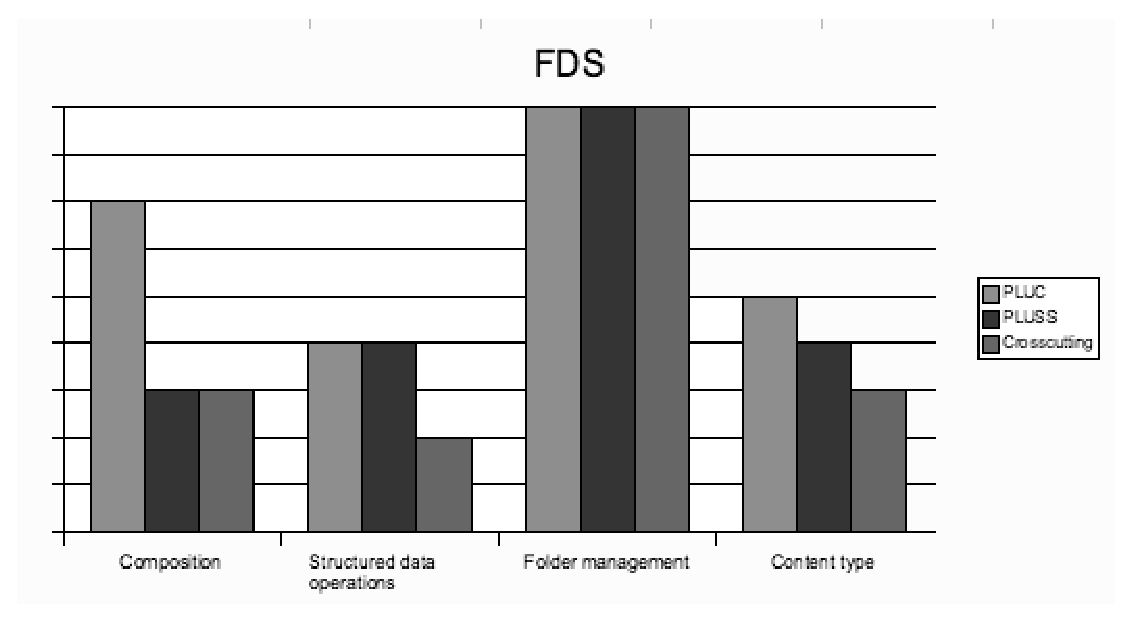
\includegraphics[scale=0.35]{img/fds-mms.eps}
  \caption{Relative FDS for evaluated techniques}
  \label{fig:fds-mms}
  \end{center}
\end{figure}
  
\subsection{Pedagogical Product Line}

We compared our approach against two specifications of the Pedagogical Product Line(PPL): the original one, proposed by the Software Engineering Institute, and a specification that was sent to us by the authors of the PLUSS technique. 

The original specification of PPL is already well modularized, since its features, in general, are not crosscutting among several use cases (see modularity metrics in Table~\ref{tab:ppl-metrics}). Moreover, another characteristic of PPL is that some features are related to qualities that do not cause effect into use cases. 

\begin{table}[hb]
\centering
\caption{PPL quantitative evaluation}
\label{tab:ppl-metrics}
\begin{small}
\begin{tabular}{lccc} \hline
					& SEI 	& PLUSS 	& Crosscutting	\\ \hline
Mean value of FDU 		& x		& 1.3	& 1.2	\\
Mean value of FDS 		& x		& 3		& 2.5	\\
Mean value of NFU 		& x		& 2		& 1.4	\\
Mean value of FSS 		& x		& 3.5	& 3		\\ 
VSU 					& 12		& 7		& 6		\\
VSS 					& 25		& 19		& 16		\\
SS 					& 44		& 38		& 32		\\	\hline
\end{tabular}
\end{small}
\end{table}

Still in this context, our approach also achieve some improvements in the resulting specifications. The main factor for these improvements in the \emph{Pedagogical} product line was the error handle modularization. Both in SEI and PLUSS specifications, the \emph{error handler} concern was spread in several use cases.    

However, by applying our approach, all behavior related to the \emph{error handler} concern was specified in a single use case. The composition of \emph{error handler} with the basic scenarios was done by means of annotations attributed to the corresponding steps. For instance, Figure~\ref{fig:error-handle} depicts just one scenario for error handling: raising  an error when there is no space available. 

\begin{figure}[h]
\begin{scriptsize}
  \texttt{
   \begin{tabular}{l}
     Description: There is no available space in file system.\\
     From step: [CatchFileException] \\
     To step: END
   \end{tabular}  
  \begin{center} 
   \begin{tabular}{|p{0.1in}|p{0.6in}|p{1.0in}|p{1.0in}|}
   \hline
       Id & User Action & System State & System Response \\ \hline \hline
       E1 & & There is not enough space to save the file. &  Raise the Disk is Full exception. The arcade game application is finished. \\  \hline
  \end{tabular}
  \end{center}
  } 
\end{scriptsize}
\caption{Scenario of error handle use case.}
\label{fig:error-handle}
\end{figure}
    
Notice that this scenario can be started from any step that has been marked with the \emph{CatchFileException} annotation (see the \emph{from step} clause). Several features of the PPL needs to save information in the file system. Therefore, both in the SEI and PLUSS specifications of \emph{Pedagogical} product line, several use cases were specified with scenarios for handling this kind of exception.


As a consequence, we achieve a significant reduction (almost 20\%) in the number of specification steps (SS in Table~\ref{tab:ppl-metrics}) when comparing to the PLUSS approach. It is important to notice that this reduction of size does not compromise the requirement coverage; but actually it means an improvement in the specification reuse.



\section{Related Work}
\label{sec:related}

Our work is linked to the body of research related to SPL
variability management, crosscutting modeling, and use case scenario
composition. This section details some of these approaches, relating
them to the proposed solution.

\subsection{Variability Management}

Pohl et al. argue that variability management should not be
integrated into existing models~\cite{phol-spl-book}. Their proposed
Orthogonal Variability Model (OVM) describes traceability links
between variation points and the conceptual models of a SPL. Our
approach can be applied in conjunction with OVM, since it also
decouple variability representation and offers a crosscutting
mechanism for specific product requirement derivation.

Hunt and McGregor proposed a pattern language for implementing
variation points~\cite{hunt-splc-2006}. The goal is to create a
catalogue that relates patterns of variabilities with good
alternatives for implementing them. It is not the goal of our work
to explicitly relate pattern variabilities with one of the proposed
mechanisms. However, our framework is also a language for
representing requirement variability mechanisms. Additionally, we
believe that it can be customized to describe mechanisms in other
SPL models.

\subsection{Crosscutting Modeling}

As result of the convergence between model driven development (MDD)
and aspect oriented software development (AOSD), several works were
proposed in order to represent weaving mechanisms using abstract
state machine and activity
diagrams~\cite{noda-aom-2006,thomas-aom-2006}. Our work, on the
other hand, describes weaving mechanisms for scenario specification
using a functional notation. First of all, we believe that the
textual language is the preferred representation for scenario
specification. Second, the use of a functional notation resulted in
a more concise model of the weaving mechanisms.

The AMPLE project aims to combine ideas from MDD and AOSD, in order
to bind the variation points at the different SPL
models~\cite{ample-url}. Our work is closed related with the AMPLE
objectives, since we describe the representation (meta-model) and
relationships between the languages involved in requirement
variability and how they crosscut each other to derive a SPL member
specification.

\subsection{Use Case Scenario Composition}

In order to avoid the problem of \emph{fragile point-cuts}, Rashid
et al. proposed a semantic approach for scenario
composition~\cite{rashid-aosd-2007}. Such approach is based on
natural language processing. Using our scenario composition weaver
(Section~\ref{sub:sc-weaver}), a scenario composition can be
represented using references to \emph{step ids} or \emph{step annotations}, 
which also reduce the problem of \emph{fragile point-cut}. However,
introducing the Rashid's approach in our environment could be
implemented without break our quantified changing mechanism. It
would be only necessary to extend the \emph{match} function
definition, called at line 3 of Listing~\ref{lst:trace}.

\section{Conclusions and Future Work}\label{sec:conclusions}

In this paper we argued about the crosscutting nature of 
variability management. Since a variant feature might require
variant points to be spread in many artifacts, it does not make sense 
to tangle variability management with the other product line artifacts. 

In order to separate variability management and scenario specification, 
we presented a crosscutting modeling framework for representing
scenario variabilities. Our approach covers two important criteria previously
defined: supporting for different kinds of variabilities and separation
of concern (SoC) between variability representation and scenario
specification. Although our modeling framework was proposed for handle 
scenario variabilities, we believe that it could be customized to be applied in 
other SPL artifacts. Particularly, optional and parameterized artifacts 
are also relevant for non-functional requirements in a product line.

As future work, we want to identify the relationship between
variabilities at different SPL artifacts (in a first moment, test
artifacts). Such kind of relationships can help in the product
generation and traceability activities of a SPL. The modeling
framework proposed in this work takes a step in this direction, since the 
composition process used to derive product specific scenarios have been already 
implemented.

%
% ---- Bibliography ----
%

\bibliographystyle{abbrv}
\bibliography{rbonifacioFSE}

\end{document}
